\documentclass[12pt,a4paper]{article}
\usepackage[utf8]{inputenc}
\usepackage{graphicx}
\usepackage{geometry}
\usepackage{hyperref}
\usepackage{tabularx}
\usepackage{caption}
\usepackage{setspace}
\usepackage{enumitem}

\geometry{top=2cm, bottom=2cm, left=2.2cm, right=2.2cm}
\setstretch{1.0}

\hypersetup{colorlinks=true, linkcolor=black, urlcolor=blue}

\begin{document}

\begin{titlepage}
\begin{center}
    \vspace*{3cm}
    \textbf{\Large LAPORAN TUGAS AUTOENCODER}\\[0.5cm]
    \textbf{\Large Rekonstruksi Citra Fashion-MNIST}\\[1.5cm]
    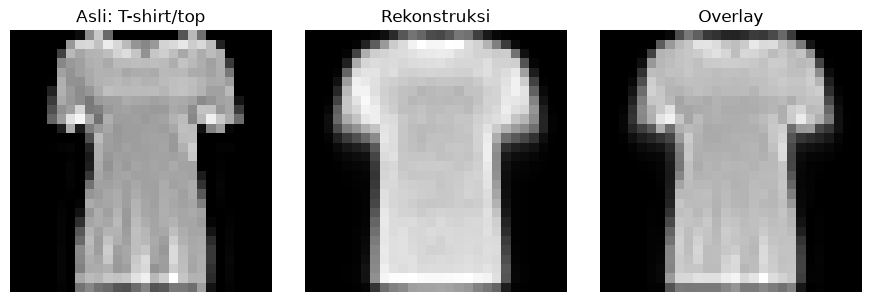
\includegraphics[width=4cm]{../hasil/comparison.png}\\[1cm]
    \textbf{Farrel Ghozy Affifudin}\\[0.2cm]
    \textbf{452024611053}\\[0.2cm]
    Teknik Informatika TI-5A2\\[0.2cm]
    Universitas Darussalam Gontor\\[2cm]
    2026
\end{center}
\end{titlepage}

\section{Pendahuluan}
Autoencoder merupakan salah satu arsitektur jaringan saraf tiruan yang belajar merekonstruksi kembali data input melalui proses kompresi dan dekompresi. Tugas ini bertujuan untuk melatih model autoencoder pada dataset Fashion-MNIST, menyimpan model hasil pelatihan, serta menjalankan proses rekonstruksi dan generasi citra melalui terminal. Eksperimen dilakukan dengan tiga variasi ukuran \textit{latent dimension}, yaitu 2, 8, dan 32, untuk menganalisis pengaruhnya terhadap kualitas rekonstruksi.

\section{Arsitektur Autoencoder}
Model autoencoder yang digunakan terdiri dari dua komponen utama:
\begin{itemize}[nosep]
    \item \textbf{Encoder}: Input 784 $\rightarrow$ Dense 256 $\rightarrow$ ReLU $\rightarrow$ Dense 64 $\rightarrow$ ReLU $\rightarrow$ Dense \textit{latent\_dim}
    \item \textbf{Decoder}: \textit{latent\_dim} $\rightarrow$ Dense 64 $\rightarrow$ ReLU $\rightarrow$ Dense 256 $\rightarrow$ ReLU $\rightarrow$ Dense 784 $\rightarrow$ Sigmoid
\end{itemize}
Loss function yang digunakan adalah \textit{Binary Cross-Entropy} (BCELoss) dengan optimizer Adam dan \textit{learning rate} $10^{-3}$. Model dilatih selama 30 epoch dengan batch size 128.

\section{Proses Training}
Training dilakukan menggunakan PyTorch dengan akselerasi GPU CUDA. Dataset Fashion-MNIST terdiri dari 60.000 gambar training dan 10.000 gambar testing berukuran $28 \times 28$ pixel dalam 10 kelas pakaian. Tiga model dilatih secara terpisah dengan latent dimension berbeda.

\begin{figure}[h!]
    \centering
    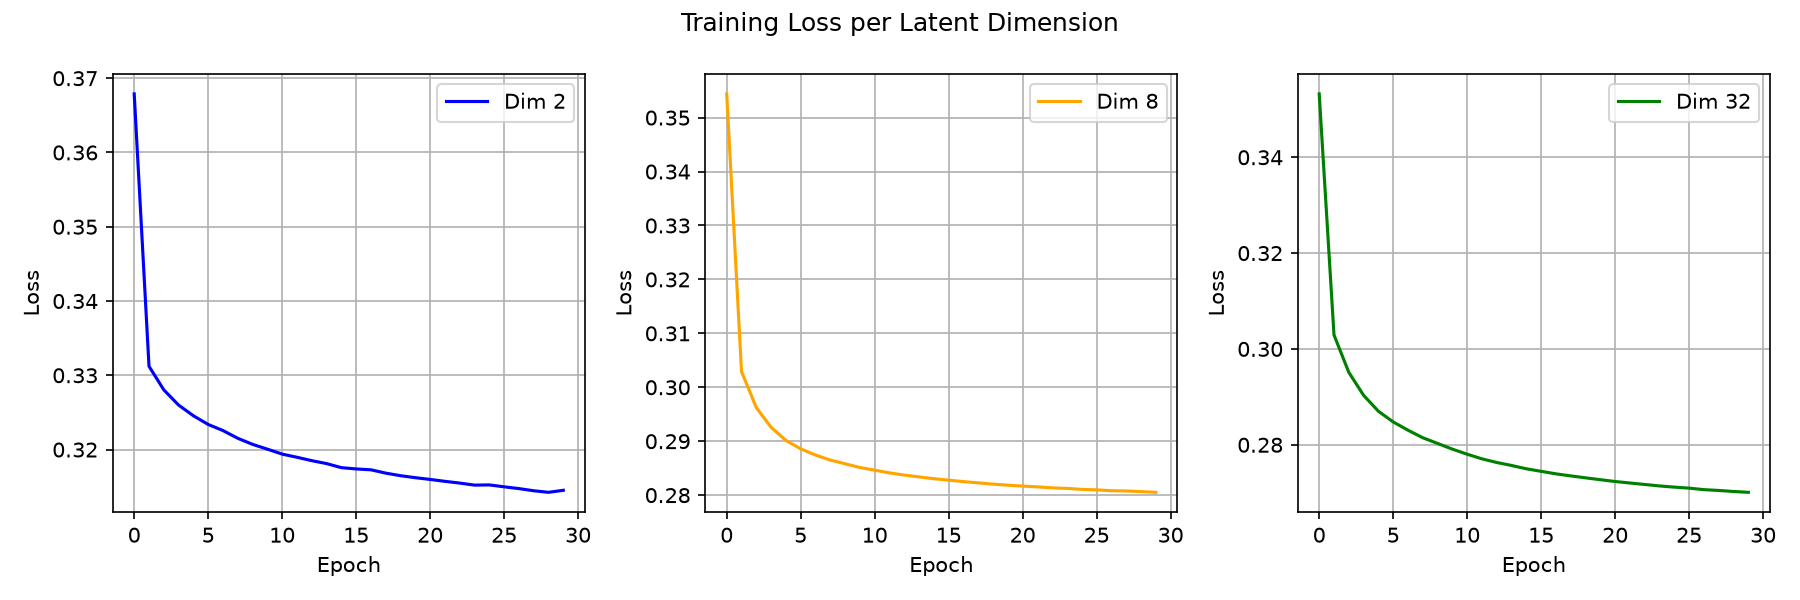
\includegraphics[width=\textwidth]{../hasil/training_loss.png}
    \caption{Grafik training loss per latent dimension}
\end{figure}

\begin{figure}[h!]
    \centering
    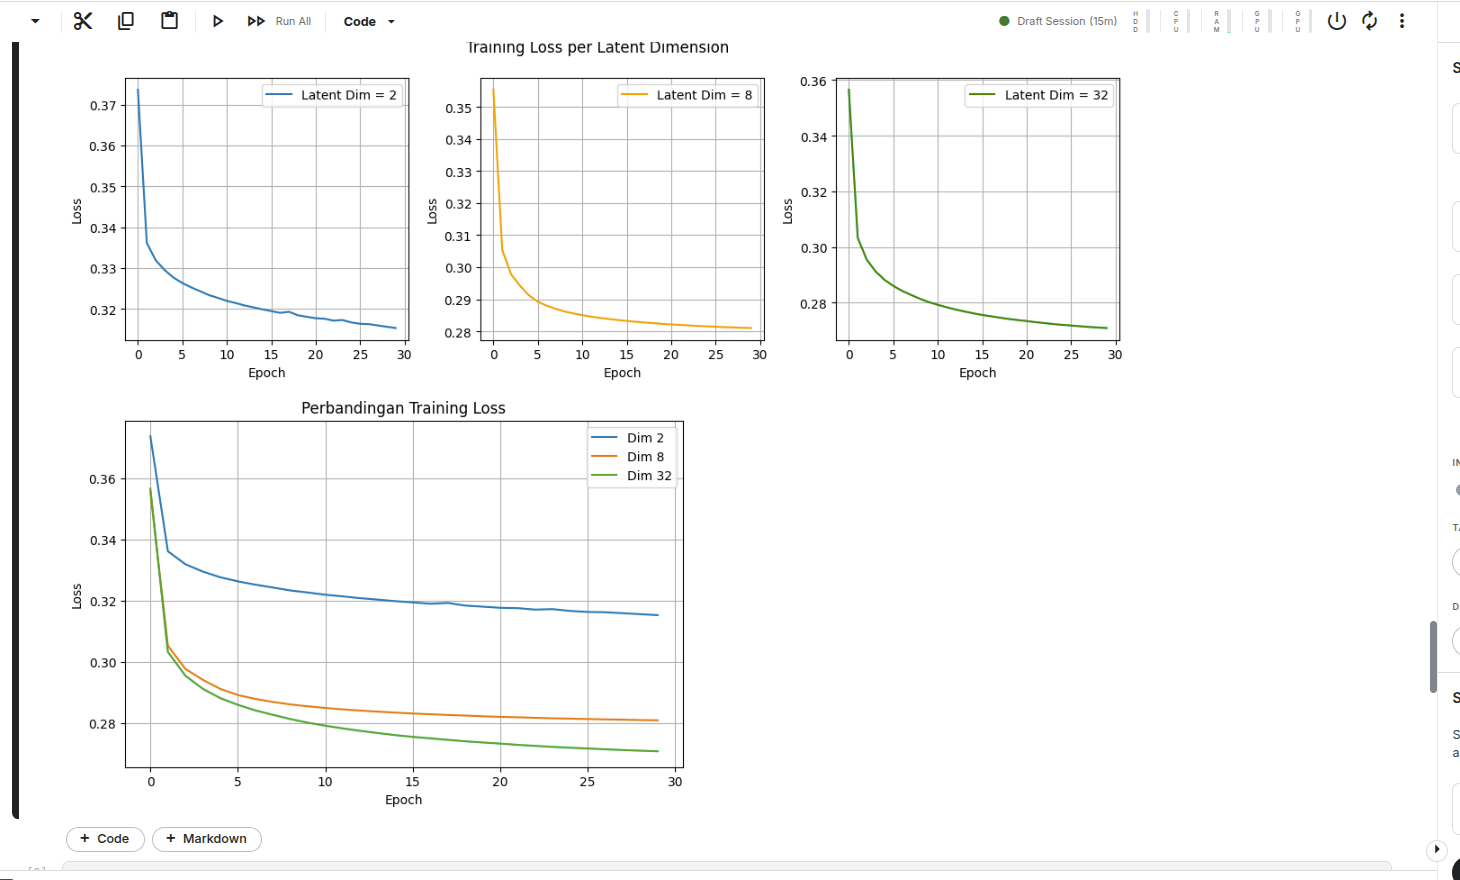
\includegraphics[width=\textwidth]{../hasil/kaggle_training.png}
    \caption{Screenshot proses training di Kaggle Notebook}
\end{figure}

\section{Tabel Perbandingan Hasil}
\begin{table}[h!]
\centering
\begin{tabularx}{\textwidth}{|c|c|c|X|}
\hline
\textbf{Latent Dim} & \textbf{Loss Akhir} & \textbf{Kualitas Visual} & \textbf{Catatan} \\
\hline
2 & 0.314519 & Buram, detail hilang & Informasi terkompresi sangat ketat \\
\hline
8 & 0.280521 & Cukup jelas & Keseimbangan kompresi dan detail \\
\hline
32 & 0.270076 & Paling tajam & Detail visual terbaik \\
\hline
\end{tabularx}
\caption{Perbandingan hasil eksperimen}
\end{table}

\section{Hasil Rekonstruksi}
\begin{figure}[h!]
    \centering
    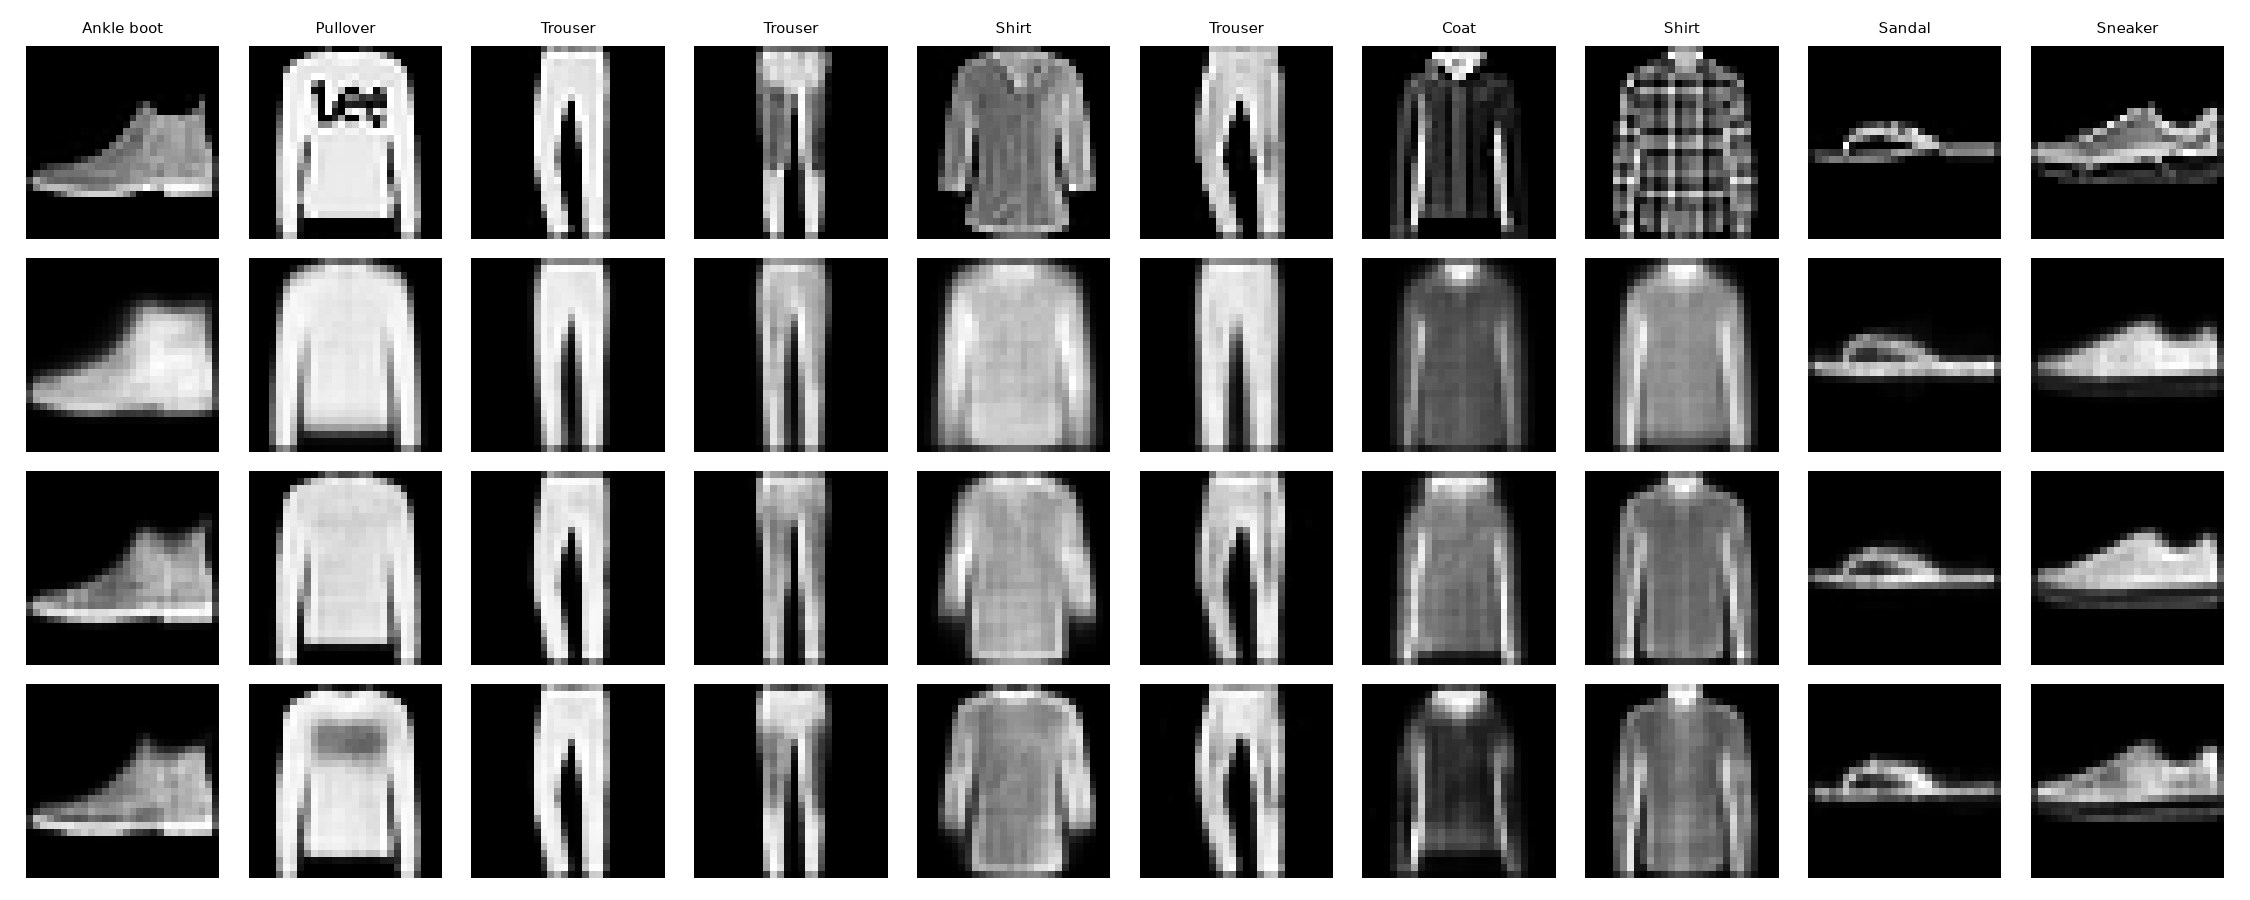
\includegraphics[width=\textwidth]{../hasil/reconstructions_comparison.png}
    \caption{Perbandingan rekonstruksi dari 10 sampel Fashion-MNIST}
\end{figure}

Gambar di atas menunjukkan perbandingan rekonstruksi untuk tiga ukuran latent dimension. Secara visual, latent dim 2 menghasilkan rekonstruksi paling buram, sedangkan latent dim 32 memberikan hasil yang paling mendekati gambar asli.

\begin{figure}[h!]
    \centering
    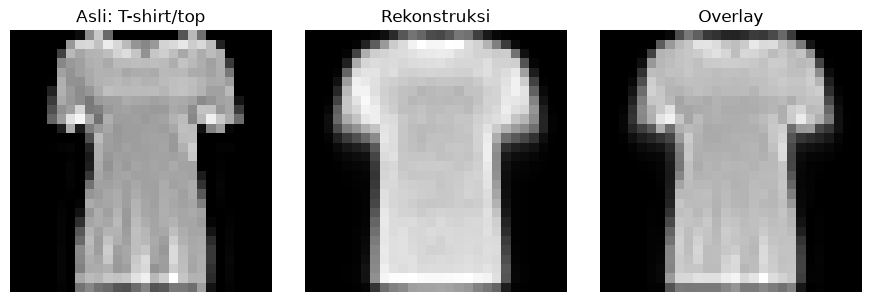
\includegraphics[width=0.6\textwidth]{../hasil/comparison.png}
    \caption{Perbandingan gambar asli, rekonstruksi, dan overlay (latent dim 2)}
\end{figure}

\section{Penjelasan Program Terminal}

\subsection{Rekonstruksi Autoencoder Penuh}
Program \texttt{reconstruct.py} digunakan untuk merekonstruksi citra dari model autoencoder lengkap.
\begin{itemize}[nosep]
    \item Argumen \texttt{--model}: path file model .pth
    \item Argumen \texttt{--index}: indeks data Fashion-MNIST
\end{itemize}
Contoh perintah:
{\small\begin{verbatim}
python scripts/reconstruct.py --model models/autoencoder_dim2.pth --index 10
\end{verbatim}}
Output: \texttt{hasil/original.png}, \texttt{hasil/reconstructed.png}, \texttt{hasil/comparison.png}

\subsection{Generasi dari Decoder}
Program \texttt{generate\_from\_decoder.py} menggunakan decoder saja untuk menghasilkan citra dari latent vector.
\begin{itemize}[nosep]
    \item Untuk latent dim 2: \texttt{--z1} dan \texttt{--z2}
    \item Untuk latent dim lebih dari 2: \texttt{--latent} sebagai daftar angka
\end{itemize}
Contoh perintah:
{\small\begin{verbatim}
python scripts/generate_from_decoder.py --decoder models/decoder_dim2.pth --z1 0.5 --z2 -1.2
python scripts/generate_from_decoder.py --decoder models/decoder_dim8.pth
  --latent "0.5,-1.2,...,0.2"
\end{verbatim}}

\subsection{Hasil Generasi Decoder}
\begin{figure}[h!]
    \centering
    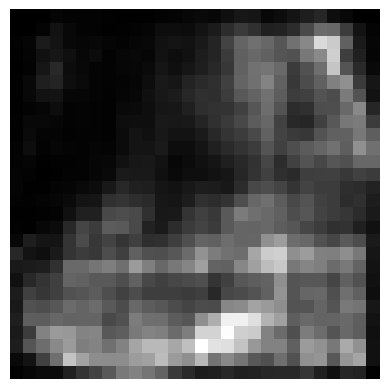
\includegraphics[width=0.25\textwidth]{../hasil/generated_dim2.png}
    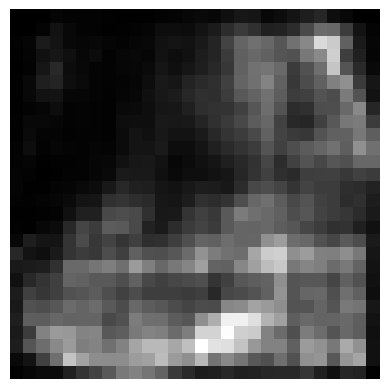
\includegraphics[width=0.25\textwidth]{../hasil/generated_dim8.png}
    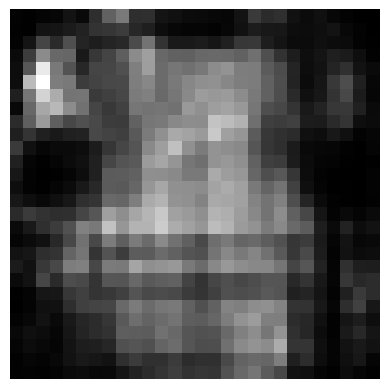
\includegraphics[width=0.25\textwidth]{../hasil/generated_dim32.png}
    \caption{Hasil generasi dari decoder dengan latent vector acak (dim 2, 8, 32)}
\end{figure}

\subsection{Screenshot Terminal}
\begin{figure}[h!]
    \centering
    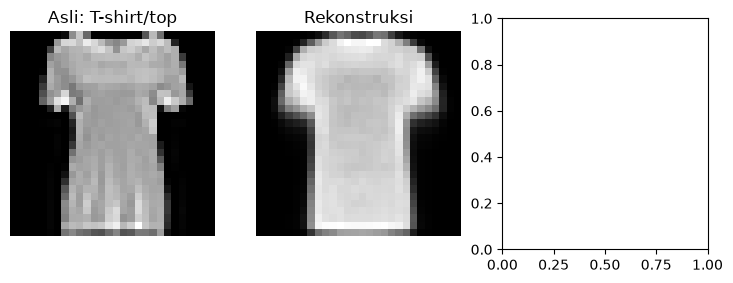
\includegraphics[width=0.9\textwidth]{../hasil/terminal_reconstruct.png}
    \caption{Screenshot terminal menjalankan \texttt{reconstruct.py}}
\end{figure}

\begin{figure}[h!]
    \centering
    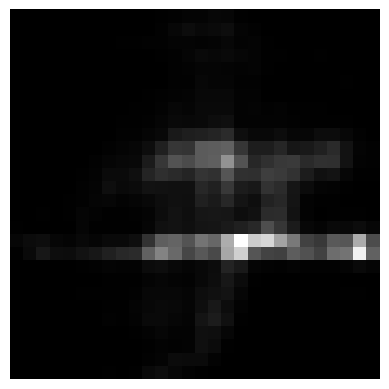
\includegraphics[width=0.9\textwidth]{../hasil/terminal_generate.png}
    \caption{Screenshot terminal menjalankan \texttt{generate\_from\_decoder.py}}
\end{figure}

\section{Analisis}
Pada model autoencoder yang dibangun, encoder berperan mereduksi citra Fashion-MNIST berdimensi 784 piksel menjadi representasi laten berdimensi lebih kecil. Proses ini memaksa model untuk menangkap fitur-fitur paling esensial dari setiap gambar, seperti kontur, pola, dan struktur visual pakaian. Representasi laten inilah yang kemudian digunakan decoder untuk membangun kembali citra ke bentuk aslinya.

Berdasarkan hasil eksperimen, latent dimension 2 menunjukkan kelemahan paling signifikan: banyak detail visual hilang sehingga hasil rekonstruksi tampak buram dan sulit dibedakan antar kelas. Hal ini terjadi karena ruang laten yang terlalu kecil tidak mampu menampung informasi yang cukup untuk merekonstruksi seluruh variasi dalam dataset. Sebaliknya, latent dimension 32 memberikan kualitas rekonstruksi paling baik dengan detail visual yang lebih tajam dan bentuk yang lebih mendekati aslinya.

Ukuran latent space secara langsung memengaruhi keseimbangan antara kompresi dan kualitas rekonstruksi. Latent dimension yang lebih besar menyediakan lebih banyak derajat kebebasan untuk menyimpan informasi fitur, sehingga decoder memiliki lebih banyak data untuk membangun kembali citra. Namun demikian, dimensi yang terlalu besar berpotensi menyebabkan model \textit{overfit} atau belajar menyalin input tanpa memahami struktur sebenarnya.

Hasil generasi dari decoder dengan latent vector acak menunjukkan bahwa decoder tidak menghasilkan citra yang bermakna secara visual. Citra yang dihasilkan tampak seperti noise atau pola abstrak yang tidak menyerupai pakaian. Ini menegaskan bahwa decoder tidak ``memahami'' struktur pakaian secara semantik, melainkan hanya memetakan koordinat dalam ruang laten ke distribusi piksel yang telah dipelajari. Latent vector acak yang berada di luar distribusi data training menghasilkan output yang tidak bermakna.

Nilai loss menunjukkan tren yang konsisten dengan kualitas visual: latent dim 2 memiliki loss tertinggi (0.3145), dim 8 menengah (0.2805), dan dim 32 terendah (0.2701). Meskipun demikian, nilai loss yang lebih rendah tidak selalu menjamin kualitas visual terbaik untuk semua metrik, karena BCELoss mengukur perbedaan pixel-wise yang tidak sepenuhnya menangkap persepsi visual manusia.

Proses rekonstruksi melalui terminal menunjukkan pentingnya konsistensi arsitektur antara training dan inferensi. Model yang disimpan dalam format .pth harus dimuat dengan arsitektur yang identik agar hasil rekonstruksi sesuai. Ketika decoder dijalankan secara terpisah, ia tetap membutuhkan latent vector sebagai input karena dalam arsitektur autoencoder, decoder tidak memiliki akses langsung ke data asli \textemdash{} ia hanya menerima output dari encoder. Hal ini menegaskan bahwa rekonstruksi merupakan rantai proses: input image $\rightarrow$ encoder $\rightarrow$ latent space $\rightarrow$ decoder $\rightarrow$ reconstructed image.

\section{Kesimpulan}
Autoencoder berhasil merekonstruksi citra Fashion-MNIST dengan kualitas yang bervariasi tergantung ukuran latent dimension. Latent dimension 32 memberikan hasil terbaik dengan loss 0.2701, sementara latent dimension 2 menghasilkan rekonstruksi paling buram dengan loss 0.3145. Autoencoder bekerja dengan memampatkan informasi ke dalam representasi laten dan kemudian merekonstruksinya kembali, bukan dengan memahami struktur gambar secara semantik. Hal ini terbukti dari hasil generasi latent vector acak yang tidak menghasilkan citra bermakna. Program rekonstruksi dan generasi decoder telah berhasil dijalankan melalui terminal dan menghasilkan file gambar sesuai ketentuan tugas.

\end{document}
